%!TEX root = ../../thirdYearReport.tex
\subsection{IIT contributions to dissemination}

\begin{figure}[!t]
	\begin{center}
		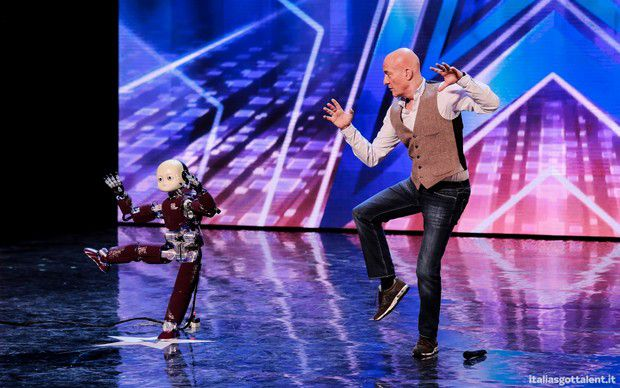
\includegraphics[width=.5\textwidth]{images/icub_igt.jpeg}		
		\caption{The iCub CoDyCo demonstration at the national television show Italia's got talent. }
		\label{fig:iCubIGT}
	\end{center}
\end{figure}

4 invited visiting periods, 4 international events participation, 12 publications (4 journal articles, 8 international conferences), several media coverage events.

\subsubsection{Invited talks}

\begin{enumerate}

\item  Event: Francesco Nori invited researcher at Tokyo University (Japan), Laboratory for Intelligent Systems and Informatics, Department of Mechano-Informatics, School of Information Science and Technology. Period: from October 1, 2015 to October 31, 2015.

\item  Event: Francesco Nori invited researcher at AIST (Japan), CNRS-AIST Joint Robotics Laboratory UMI3218/RL (JRL) situated at the Intelligent Systems Research Institute (IS), National Institute of Advance Industrial Science and Technology (AIST). Period: from November 15, 2015 to December 6, 2015.

\item  Event: Francesco Nori invited researcher at Université Paris Sud (France). University Paris Sud 11, Paris. CIAMS laboratory in the Motor Control and perception team, University Paris-Sud 11, Paris, France. Inviting professors: Prof. Bastien Berret, University Paris-Sud 11 and Prof. Fr\'ed\'eric Jean, ENSTA Paris-Tech, Unit\'e de Math\'ematiques Appliqu\'ees. Period: from June 1, 2015 to June 30, 2015.

\item  Event: Francesco Nori invited researcher at INRIA, Nancy (France). Serena Ivaldi invited Francesco Nori from January 25th to Febraury 19th to spend a visiting periodo at team Larsen, INRIA. Inviting researcher: Serena Ivaldi. Period: from January 25th to Febraury 19th, 2016. During this visiting period Francesco and Serena planned the activities for the fourth year demonstration.
\end{enumerate}

\subsubsection{International events participation}

\begin{enumerate}

\item The iCub Summer School, ``Veni Vidi Vici'', serves to consolidate and disseminate skills in software engineering for humanoid robots. Our goal is to foster collaboration on robot software across the boundaries and lifetimes of specific platforms and projects.
The school focuses on humanoid robotics and will host at least two iCub and a COMAN robot. Students will receive an initial training on the software infrastructure (middleware and tools) and will be required to work on a project of their choice. All participants are expected to be competent C/C++ programmers with an interest in working with others (and an agenda of their own). Info: \url{http://wiki.icub.org/wiki/VVV15}

\begin{figure}[!t]
	\begin{center}
		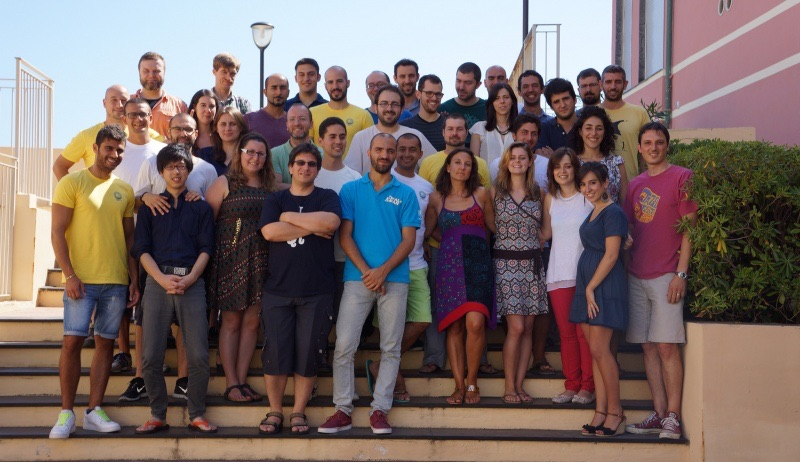
\includegraphics[height=4.5cm]{images/vvv.jpg}
		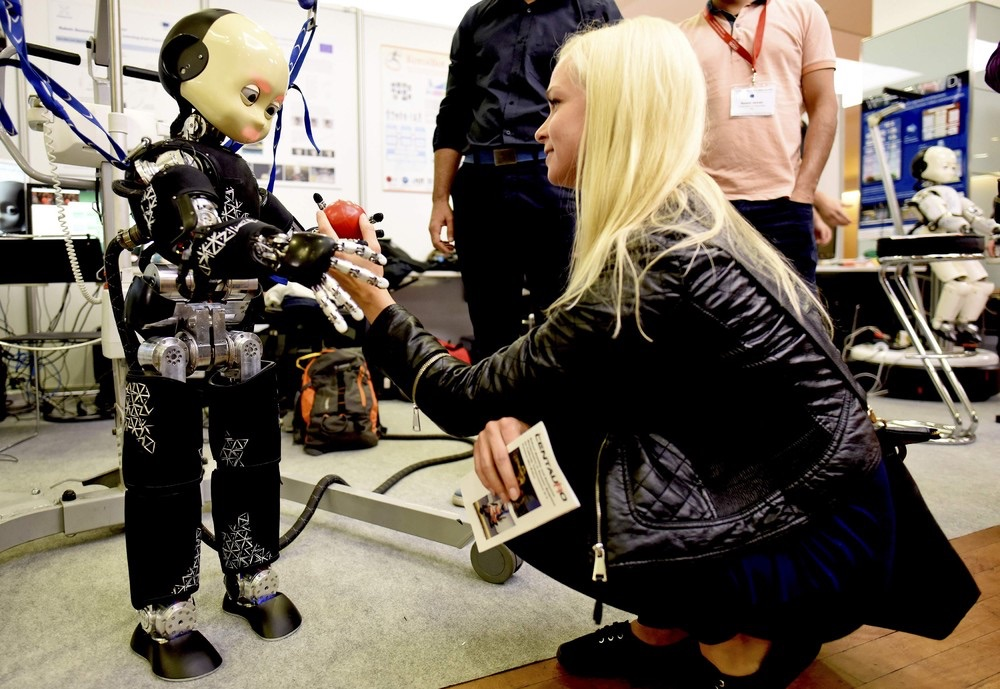
\includegraphics[height=4.5cm]{images/iros.jpg}
        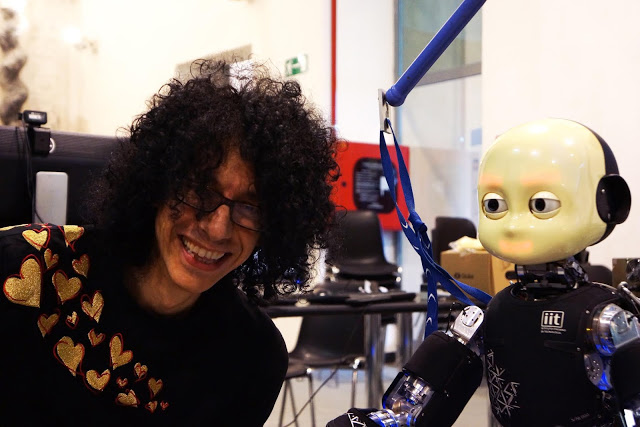
\includegraphics[height=4.5cm]{images/allevi.jpg}
        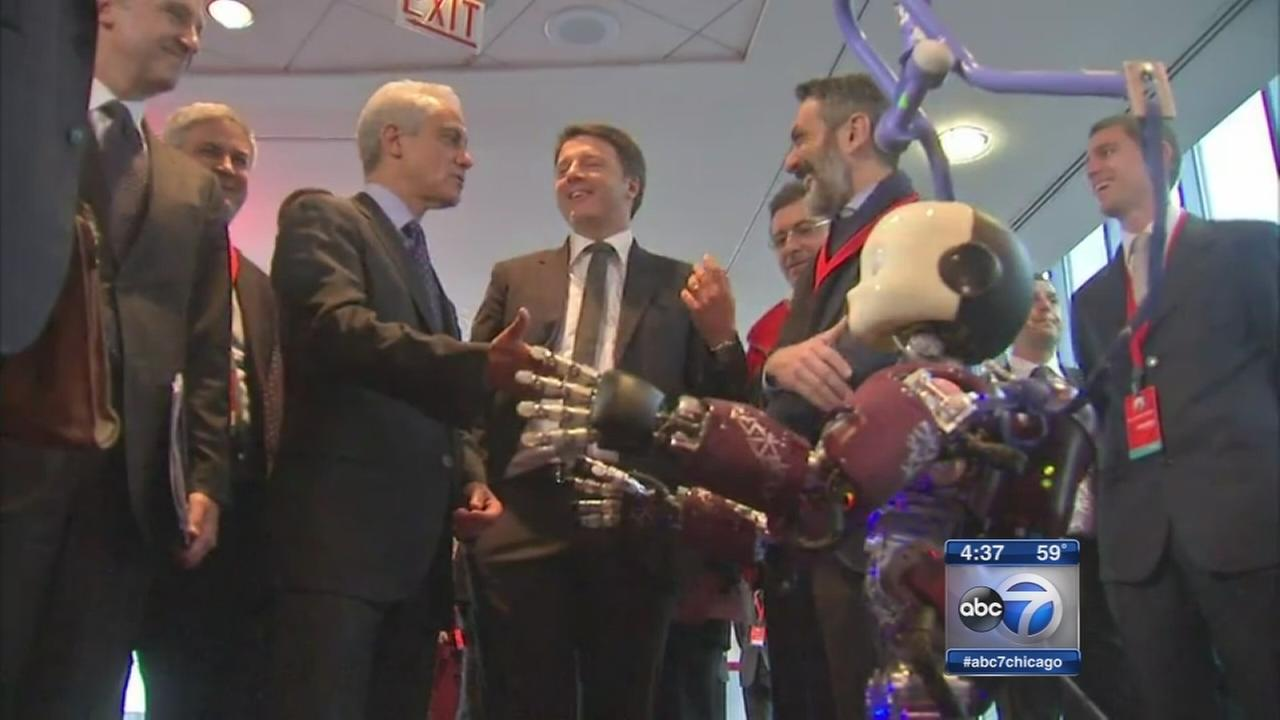
\includegraphics[height=4.5cm]{images/renzi.jpg}
		\caption{Top left: the iCub Veni-Vidi-Vici summer school. Top right: the iCub at the IROS 2015 event organised by the robotics unit at the European Commission. Bottom left: iCub with the piano player, Giovanni Allevi. Bottom right: icub with Matteo Renzi at the ``Italian Manufacturing Forum''. }
		\label{fig:vvv}
	\end{center}
\end{figure}

\item During the IROS 2015 International Conference at Hamburg, different versions of iCub (the Genova Black, and the Heidelberg version) were shown in an exhibition. For three days, iCub interact with visiting people performing different demos, such as torque balancing and the red ball demo. Photo by Fabian Bimmer/Reuters)

\item In July, during the RSS conference in Rome, a full day workshop titled ``Towards a Unifying Framework for Whole-body and Manipulation Control'' has been organised. Topics covered the following areas: contacts planning and control; whole-body task control; compliant whole-body movements; dynamics in humanoid robots; machine learning and optimization methods for contact planning and control.

\item Live demonstrations at the event: ``Italian Manufacturing Forum'', UIC Gleacher Center, Chicago, IL, March 30th, 2016. The iCub was shipped to Chicago to perform several iCub related demonstrations (e.g. iCub standing, iCub performing whole-body equilibrium tasks) at the Italian Manufacturing Forum. 
\end{enumerate}

\subsubsection{Other events}

\begin{enumerate}

\item iCub has been a special guest in Ballar\'o, an italian political show on the public television network. The video of the event is available here: \url{https://youtu.be/DE3VynOr6HE}.

\item In May, Francesco Nori was an invited speaker at the Creative Mornings event. The talk gave historical and philosophical motivations that guided recent research activities towards the problem of studying how humans interact with the environment and among themselves. The iCub was also presented, as an open-source platform capable of advancing the state-of-the-art in various directions, e.g. decisional autonomy, dependability/adaptability, perception and, in a single all-embracing word, cognitive abilities.

\item From 22nd of October to 1st of November 2015, the iCub will be showed at the ``Festival della Scienza''. Festival della Scienza, now at its 13th edition, is a publicly opened event which focus on science. During this festival, temporary laboratories and exhibition booths are prepared where researchers and scientists can show and explain to people their work. Presentations are targeted to different audiences, from children to university students to adults. This year festival theme is ``Equilibrium'', and iCub will perform daily showing balancing demos. 

\item Live video shooting at ``Italia's got talent'', italian national television show. Shooting: December 1st-3rd 2015. Location: Catanzaro, Italy. The iCub performed the CoDyCo demo based on whole-body torque controlled motions with switching motions.
\end{enumerate}

\subsubsection{Talks at international conferences}

\begin{enumerate}
\item Event: invited talk at the dissemination event Creative mornings. Talk: Interacting with Humans with iCub-humanoid. Dates: Location: May 22nd 2015. Milano, Italy.
\item  Event: Convegno NanoItaly, Roma, 21-24 settembre 2015. Talk: Force and motion capture system
based on distributed micro-accelerometers, gyros, force and tactile sensing. Date: 21 settembre 2015.
\item  Event: International Conference on Humanoid Robotics, 02-06 November 2015. Workshop on Benchmarking bipedal functions of humanoids robots: towards a unified framework. Talk: wholeBodyInterface: a software abstraction layer for benchmarking whole-body motion control. Date: November 3rd 2015.
\item  Event: International Conference on Humanoid Robotics, 02-06 November 2015. Workshop on Reusable and Open-Source Modules for Humanoid Robots. Talk: wholeBodyInterface: An Open- Source Software Abstraction Layer for Whole-Body Motion Control. Date: November 3rd 2015.
\item  Event: International Conference on Humanoid Robotics, 02-06 November 2015. Workshop on Whole-Body Multi-Task Multi-Contact Humanoid Control. Talk: iCub whole-body control through force regulation on rigid non-coplanar contacts. Date: November 3rd 2015.
\item  Invited external member and president at Ph.D. defense Université d'Orléans (France). Ph.D. candidate: Adina Panachea. Date: December 10th, 2015.
\end{enumerate}


\subsubsection{Pubblications}

\begin{enumerate}
\item Camoriano R., Traversaro S., Rosasco L., Metta G. \& Nori F. 2016, ‘Incremental Semiparametric Inverse Dynamics Learning’, IEEE International Conference on Robotics and Automation (ICRA), Stockholm, Sweden, May 16-21, 2016.

\item Del Prete A., Mansard N., Ramos O., Stasse O. \& Nori F. 2015, ‘Implementing Torque Control with High-Ratio Gear Boxes and without Joint-Torque Sensors’, International Journal of Humanoid Robotics.

\item Del Prete A., Nori F., Metta G. \& Natale L. 2015, ‘Prioritized Motion-Force Control of Constrained Fully-Actuated Robots: “Task Space Inverse Dynamics”’, Robotics and Autonomous Systems, vol. 63, Part 1, pp. 150–157.

\item Eljaik J., Kuppuswamy N. \& Nori F. 2015, ‘Multimodal sensor fusion for foot state estimation in bipedal robots using the Extended Kalman Filter’, IEEE/RSJ International Conference on Intelligent Robots and Systems (IROS), Hamburg, Germany, October (29 September - 1 October, 2015).

\item Latella C., Kuppuswamy N. \& Nori F. 2015, ‘Force and motion capture system based on distributed micro-accelerometers, gyros, force and tactile sensing’, 2nd International Electronic Conference on Sensors and Applications,.

\item Nori F., Kuppuswamy N. \& Traversaro S. 2015, ‘Simultaneous state and dynamics estimation in articulated structures’, IEEE/RSJ International Conference on Intelligent Robots and Systems (2015), Hamburg, Germany, October (29 September - 1 October, 2015).

\item Nori F., Traversaro S., Eljaik J., Romano F., Del Prete A. \& Pucci D. 2015, ‘iCub whole-body control through force regulation on rigid non-coplanar contacts’, Frontiers in Robotics and AI.

\item Paikan A., Traversaro S., Nori F. \& Natale L. 2015, ‘Generic Testing Framework for Test Driven Development of Robotic Systems’, in Jan Hodicky (ed.),Modelling and Simulation for Autonomous Systems Workshop, Springer International Publishing pp.216-225, , Prague, Czech Republic, 2015.

\item Pucci D., Romano F. \& Nori F. 2015, ‘Collocated Adaptive Control of Underactuated Mechanical Systems’, IEEE Transactions on Robotics.

\item Romano F., Del Prete A., Mansard N. \& Nori F. 2015, ‘Prioritized Optimal Control: a Hierarchical Differential Dynamic Programming approach’, IEEE International Conference on Robotics And Automation, Seattle, Washington, USA.

\item Traversaro S., Del Prete A., Ivaldi S. \& Nori F. 2015, ‘Inertial parameters identification and joint torques estimation with proximal force/torque sensing’, IEEE International Conference on Robotics and Automation, Seattle, USA, May 26th - 30th, 2015.

\item Traversaro S., Pucci D. \& Nori F. 2015, ‘In Situ Calibration of Six-Axis Force-Torque Sensors using Accelerometer Measurements’, IEEE International Conference on Robotics and Automation, pp.6,  Seattle, USA, May 26th - 30th, 2015.
\end{enumerate}
	
\subsubsection{Media coverage}

\begin{itemize}

\item \url{https://youtu.be/DE3VynOr6HE}

\item \url{https://youtu.be/mLqEkGwGxm0}

\item \url{https://youtu.be/RBP4BvW4RBs}

\item \url{https://youtu.be/RRg1yV_qKvY}

\item \url{https://www.facebook.com/IITalk/videos/10156433813675384/}

\item \url{https://youtu.be/im5k85_6t6s}

\end{itemize}

\subsubsection{iCub at international events}

\begin{itemize}
\item CISCO conference Milano 26/1/2015
\item Geo \& Geo Roma 25/2/2015
\item ERF Vienna, workshop on humanoids in the laboratory (chimica, ecc.) 12/3/2015
\item ITURO conference Istanbul, keynote 11/4/2015
\item CSIFT Shanghai, investors presentation 22-24/4/2015
\item Bal Robotov, invited forum on robotics, Mosca 29/4/2015
\item Robobusiness, invited, Milan 30/4/2015
\item Boston Woodshole, summer school CBMM, Robotics Afternoon, 18-22/8/2015
\item Sky International, TV, 25/8/2015
\item Uno Mattina, Rai1, 1/9/2015
\item Rai Petrolio, 10/9/2015
\item Researchers night, invited, L'Aquila 26/9/2015
\item Trieste Next Fest, invited, Trieste 27/9/2015
\item IROS, Hamburg 28/9, 2/10/2015
\item Italian Manufacturing Forum, Chicago, IL, 30/03/2016
\end{itemize}